\documentclass{article}
\usepackage{graphicx}
\usepackage{amsmath}
\usepackage{subcaption}
\usepackage{amsfonts}
\usepackage[makeroom]{cancel}

\title{TEK5600 - Obligatory Assignment}
\author{Edvart G. Bjerke}
\date{March 2025}

\begin{document}

\maketitle

\section{Field Lines}
A field line is both a mathematical object and a tool commonly used to visualize
vector fields. Field lines are curves that are tangent to the underlying vector field
at all points. The vector field defines a system of first-order differential equations, and the field lines are particular solutions to this system.

In this report, the vector field in question is a time-independent \\
2-dimensional vector field representing velocity.
Given an initial position, the field line is a parametric curve that represents the streamline of the flow, showing the path of an imaginary particle.

In practice, the solutions are not found analytically, but are simulated using 
numerical integration schemes on a discretized version of the vector field.
In this case, the domain of the vector function is discretized into an $N \times M$ grid of points.
The values at the exact grid points are samples of the true vector fields. To be able to
sample in between grid points, an interpolation scheme is used. For this project,, bilinear interpolation has been implemented. 

\begin{figure}[h!]
    \centering
    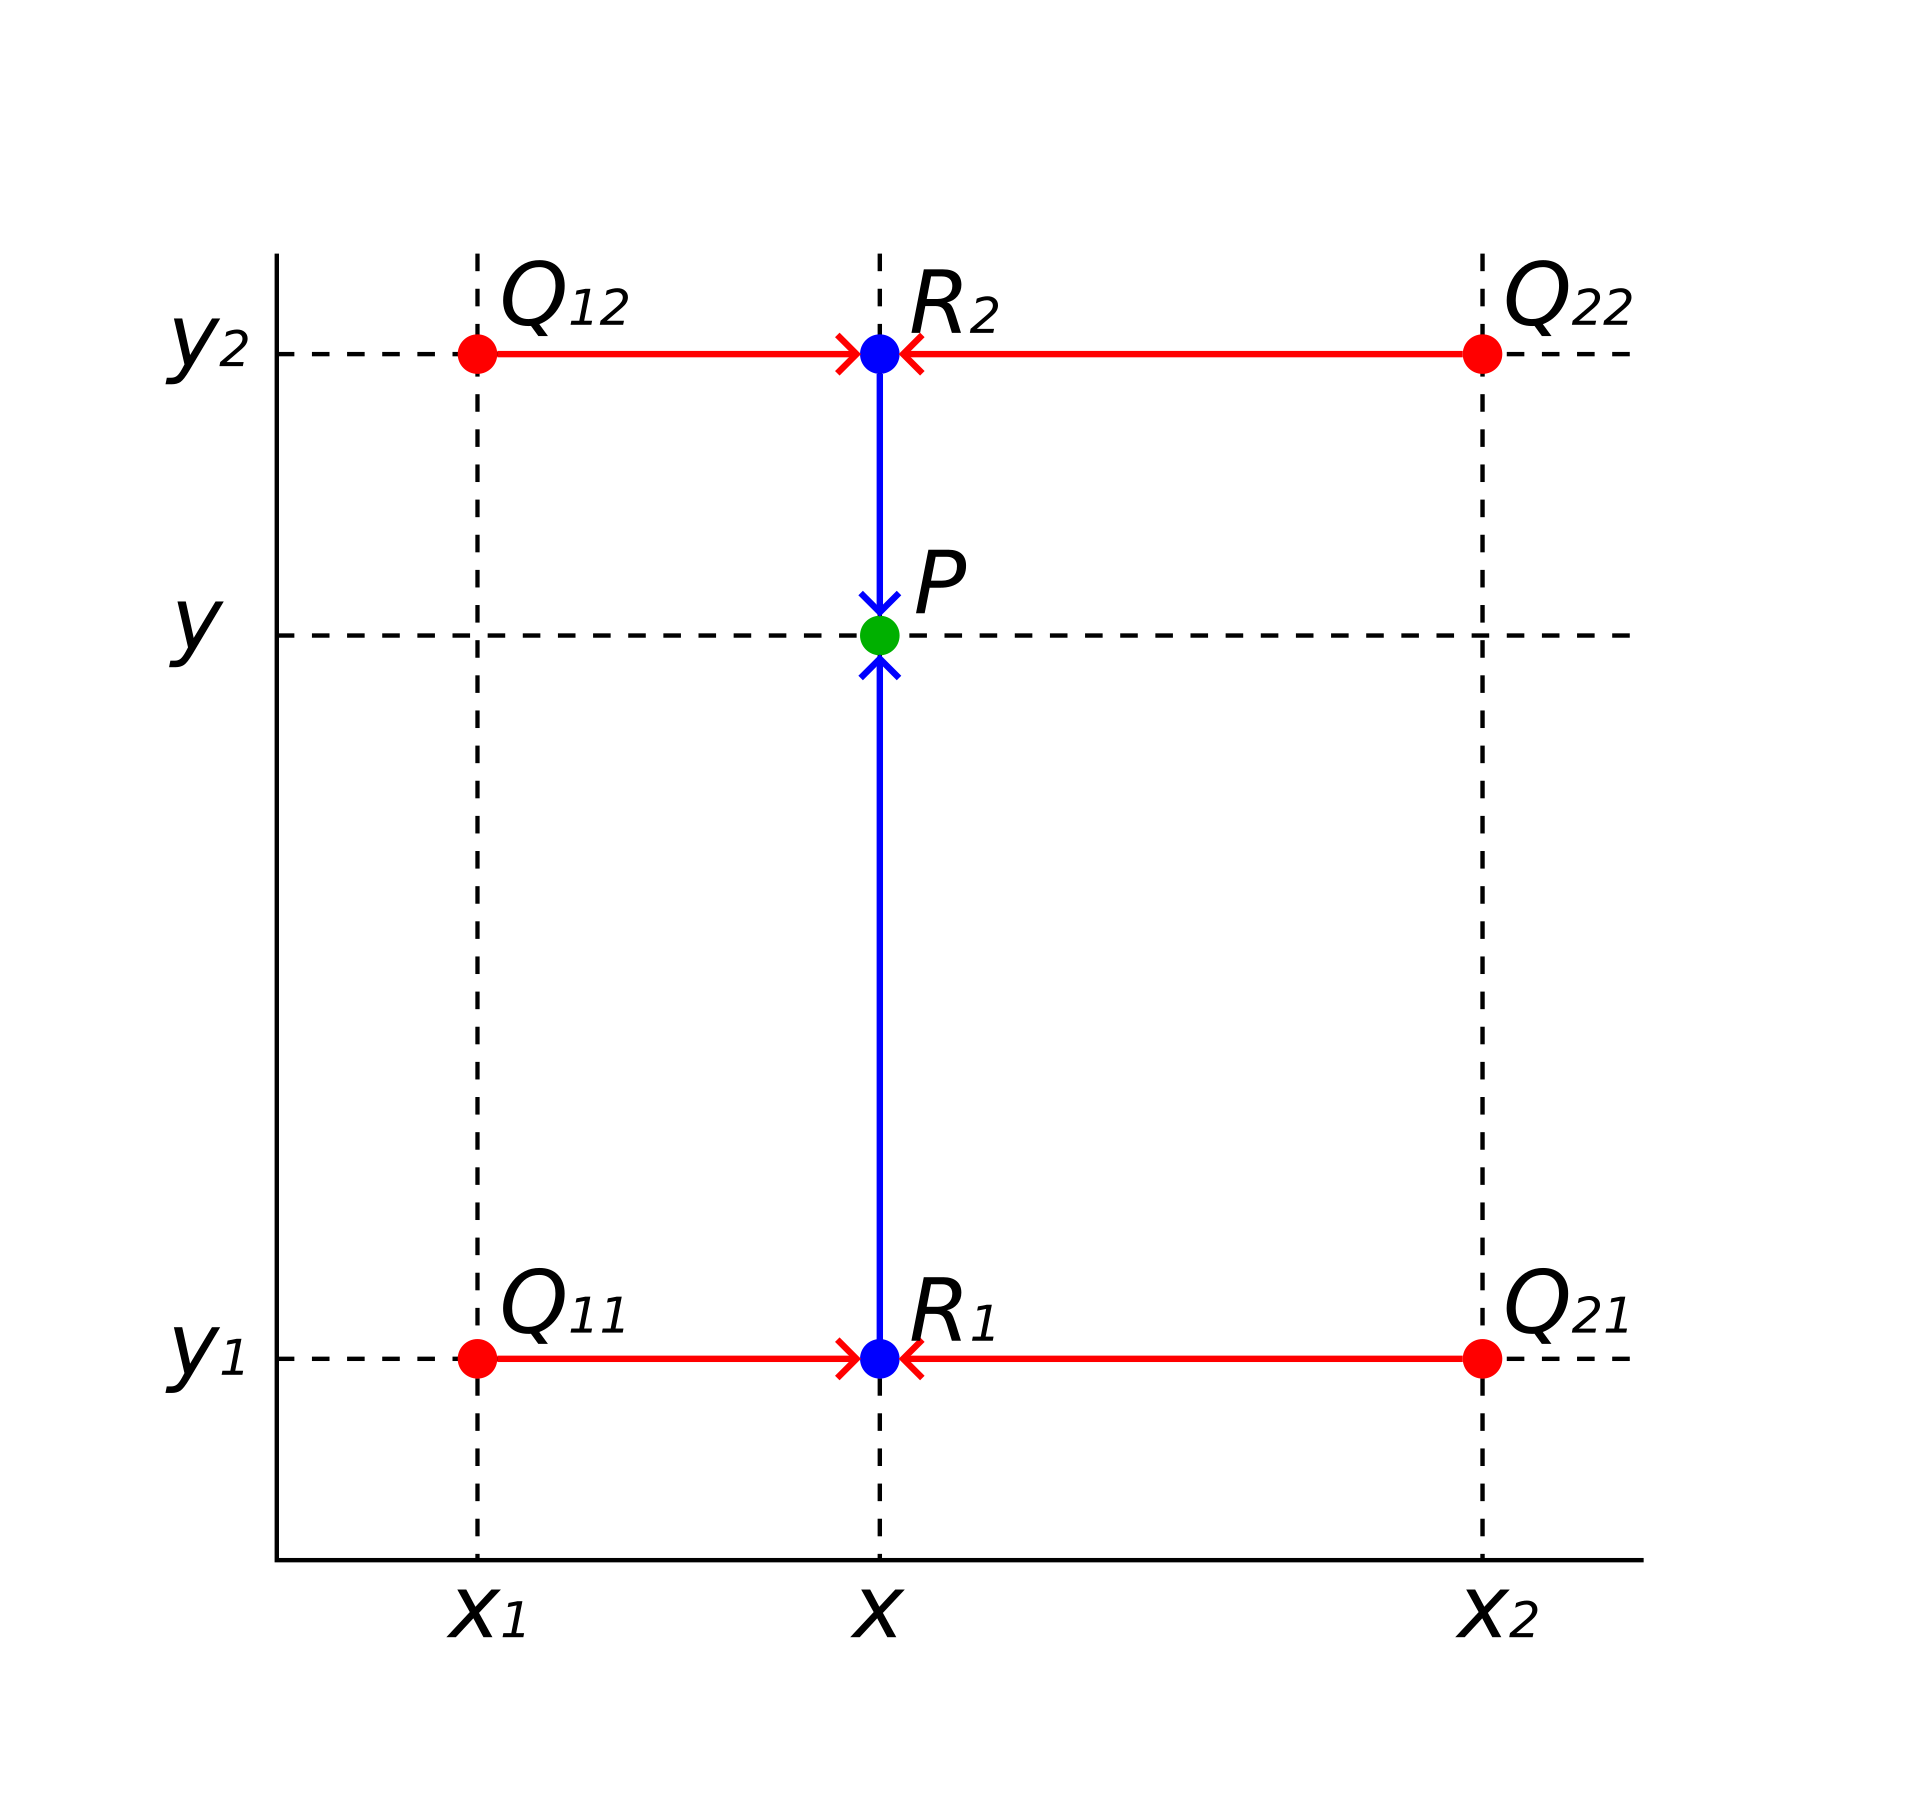
\includegraphics[width=0.5\textwidth]{BilinearInterpolationV2.svg.png}
    \caption{Bilinear interpolation. The sampled point $P$ is a weighted sum of the four nearest grid points.}
\end{figure}

\subsection{Integration schemes}
Two integration schemes were used to find particular solutions: the forward euler method and the runge-kutta (RK4) method.

The (time-independent) vector field $V$ is defined as a function which takes in a position vector  $(x, y)$, and returns a velocity vector $(u, v)$ representing the velocity at that position:
$$V : \mathbb{R}^2 \rightarrow \mathbb{R}^2 $$
$$\mathbf{V}(\mathbf{x}(t)) = \begin{bmatrix}
    u(\mathbf{x}(t)) \\
    v(\mathbf{x}(t))
\end{bmatrix}, \quad
\mathbf{x} = \begin{bmatrix}
    x\\y
\end{bmatrix}
$$

The velocity field V represents the ordinary differential equation relating 
the position vector $\mathbf{x}$ and its derivative:
$$\mathbf{x}'(t) = V(\mathbf{x}(t))$$
With solution:
$$\mathbf{x}(t) = \mathbf{x}(t_0) + \int_{t_0}^{t} \mathbf{V}(\mathbf{x(\tau)}) d\tau$$
Equations on this formed can be solved numerically using the forward euler method and RK4.

The euler method is derived by taking the first-order taylor approximation around $t = t_0$:
\begin{align*}
    \mathbf{x}(t) &\approx \mathbf{x}(t_0) + \mathbf{V}(\mathbf{x}(t_0))(t-t_0)\\
    &= \mathbf{x}(t_0) + h\mathbf{V}(\mathbf{x}(t_0)) 
\end{align*}
Where $h = (t-t_0)$ is the "step length". The error of the solution decreases as the step length is reduced.
The equation is solved iteratively by integrating one "step ahead" at a time:
$$\mathbf{x}_{k+1} = \mathbf{x}_k + hV(\mathbf{x}_k)$$

RK4 is similar to the euler method, but evaluates the derivative four times for each integration step:
$$\mathbf{x}_{k+1} = \mathbf{x}_k + \frac{h}{6}(k_1+k_2+k_3+k_4)$$
$$k_1 = \mathbf{V}(\mathbf{x}_k)$$
$$k_2 = \mathbf{V}\left(\mathbf{x}_k+\frac{h}{2}k_1\right)$$
$$k_3 = \mathbf{V}\left(\mathbf{x}_k+\frac{h}{2}k_2\right)$$
$$k_4 = \mathbf{V}\left(\mathbf{x}_k+hk_3\right)$$

\subsection{Seeding strategies}
The seeding strategy is the scheme used to select initial positions for the numerical DE solver. 
A good seeding strategy is one that is fast and captures the most important features without causing clutter.
For this assignment, three seeding strategies have been implemented.

\subsubsection{Random seeding}
Random seeding is a simple strategy where seed points are generated randomly based on some distribution.
Here, a uniform distribution was used to generate positions spanning the size of the grid.
\begin{verbatim}
for i in range(num_particles):
    seeds_x.append(np.random.random() * u.shape[0] - 2)
    seeds_y.append(np.random.random() * u.shape[0] - 2)
\end{verbatim}

\begin{figure}[h!]
    \centering
    \includegraphics[width=0.75\textwidth, angle=270]{random.png}
    \caption{Field lines from 1000 randomly distributed particles}
\end{figure}

\subsubsection{Uniform seeding}
Uniform seeding is another simple seeding strategy where seeds
are uniformly distributed (evenly spaced) onto the domain.
\begin{figure}[h!]
    \centering
    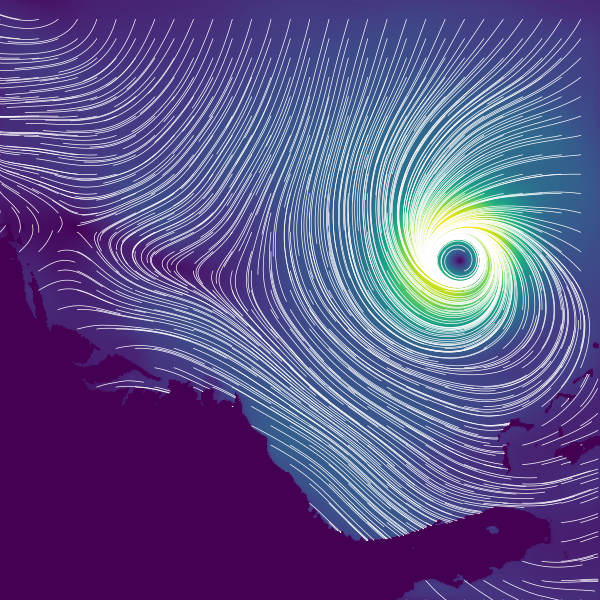
\includegraphics[width=0.75\textwidth, angle=270]{uniform.png}
    \caption{Field lines from 1000 evenly distributed particles}
\end{figure}

\subsubsection{Vorticity-based seeding}
In this custom seeding strategy, the vorticity of the vector field is used
to generate seeding points. The vorticity $\mathbf{\omega}$ is defined as the curl of the velocity field:
\begin{align*}
    \mathbf{\omega} &= \nabla \times \mathbf{v} \\
    &= \nabla \times \left[u(x, y), v(x, y)\right] \\
    &= \frac{\partial v}{\partial x} - \frac{\partial u}{ \partial y}
\end{align*}
The vorticity of a 2-dimensional velocity field is a vector field pointing purely in the z-direction. In this implementation, 
the magnitude of this vector field is used to generate a probability probability map from which seed points are randomly sampled.
Gaussian blurring has been applied to the vorticity map and a bias has been added such that even areas with close to zero vorticity are 
represented in the field line visualization.

One can also experiment with modifying the vorticity map using the power operator. Powers greater than 1 will increase the contrast
(highlight the center of the tornado) while powers less than one will equalize the vorticity map.

To compute the vorticity map, the \verb|np.gradient()| was used, which computes the derivatives of the velocity field
using second order central differences.


\begin{figure}[h!]
    \centering
    \begin{subfigure}{0.32\textwidth}
        \centering
        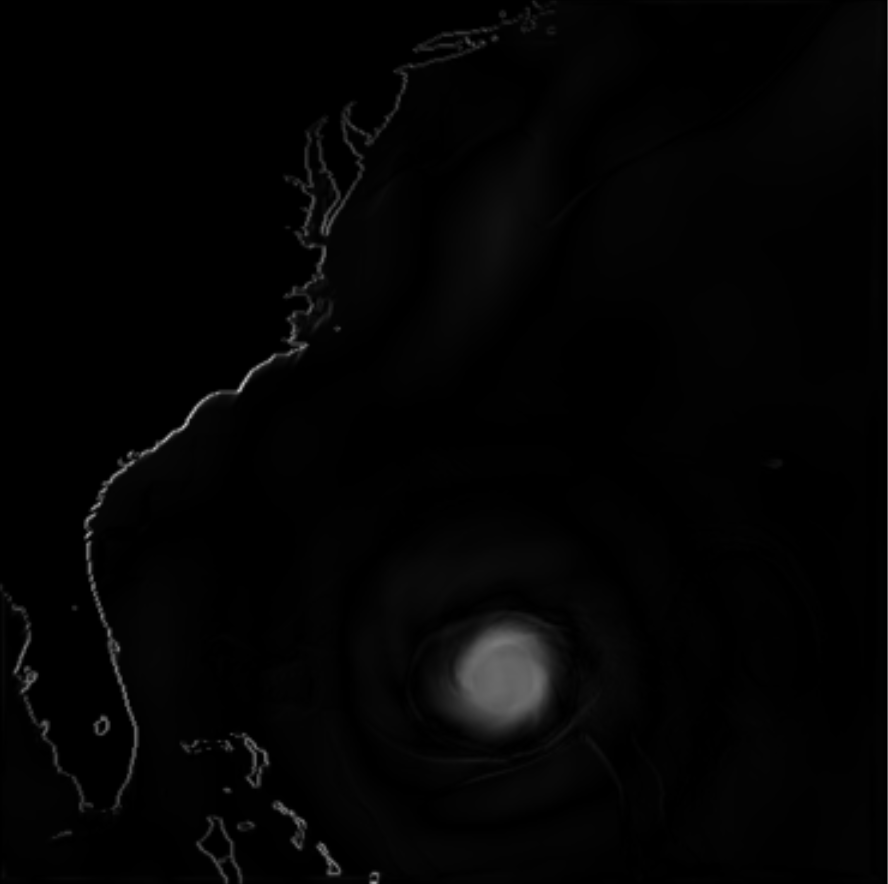
\includegraphics[width=\textwidth]{vorticity_map.png}
        \caption{Vorticity magnitude field.}
    \end{subfigure}
    \hfill
    \begin{subfigure}{0.32\textwidth}
        \centering
        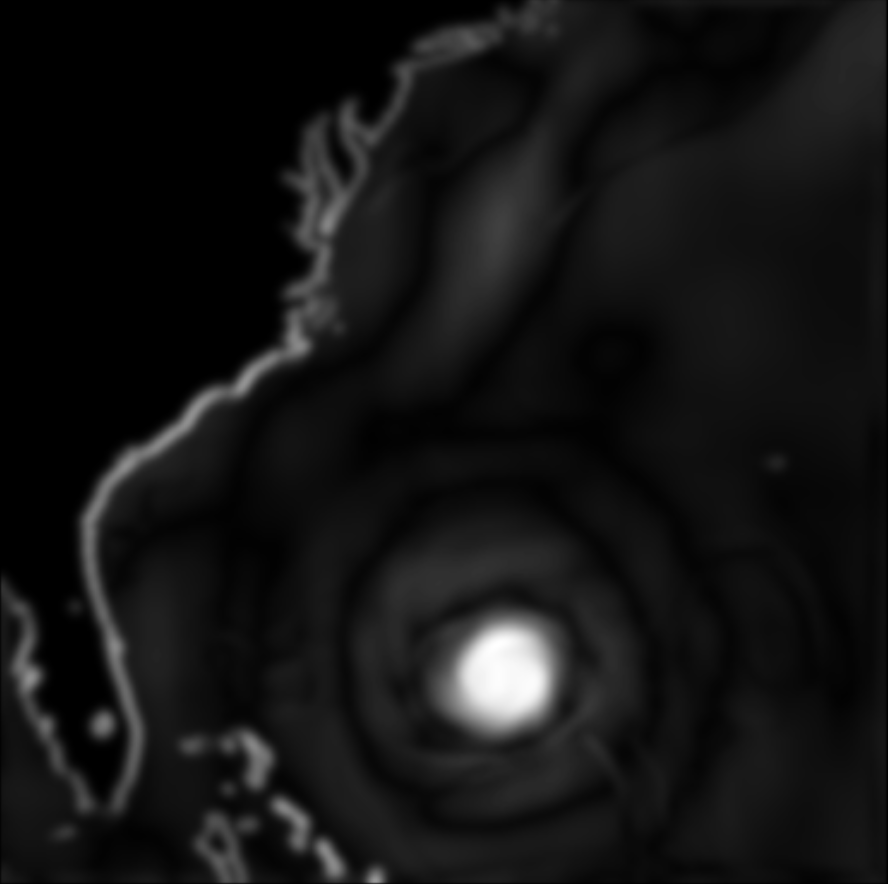
\includegraphics[width=\textwidth]{pow_0_6.png}
        \caption{Vorticity magnitude raised to 0.6.}
    \end{subfigure}
    \hfill
    \begin{subfigure}{0.32\textwidth}
        \centering
        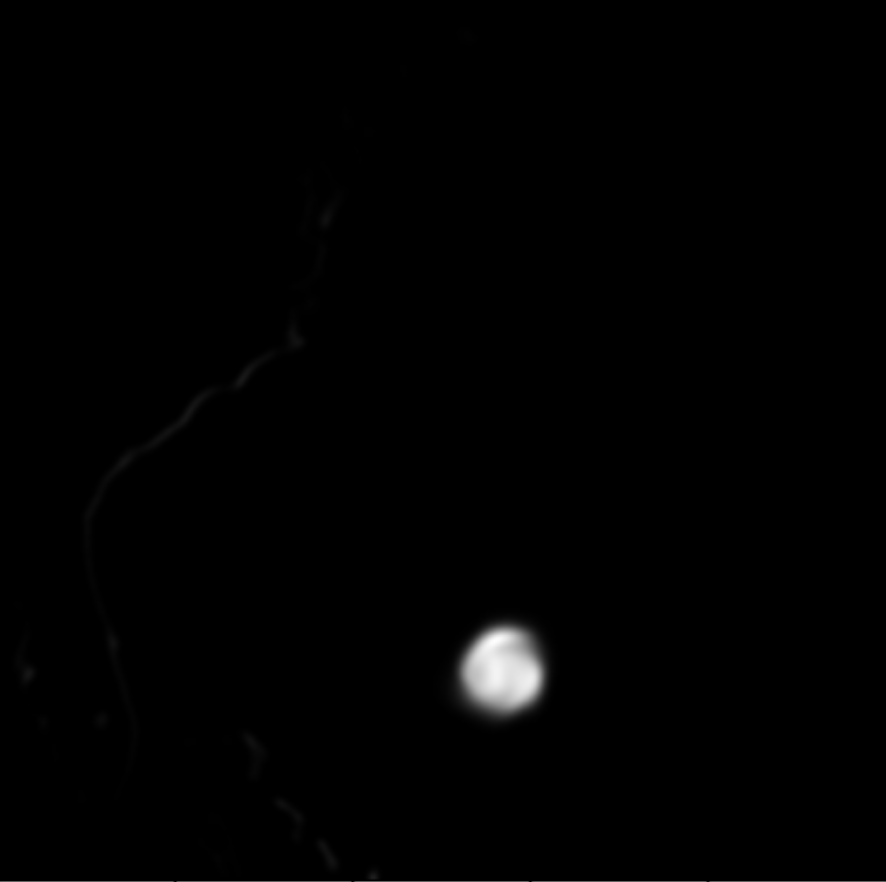
\includegraphics[width=\textwidth]{pow_3_0.png}
        \caption{Vorticity magnitude raised to 3.0.}
    \end{subfigure}
    \caption{Comparison of vorticity magnitude field transformations.}
\end{figure}



\begin{figure}[h!]
    \centering
    \begin{subfigure}{0.43\textwidth}
        \centering
        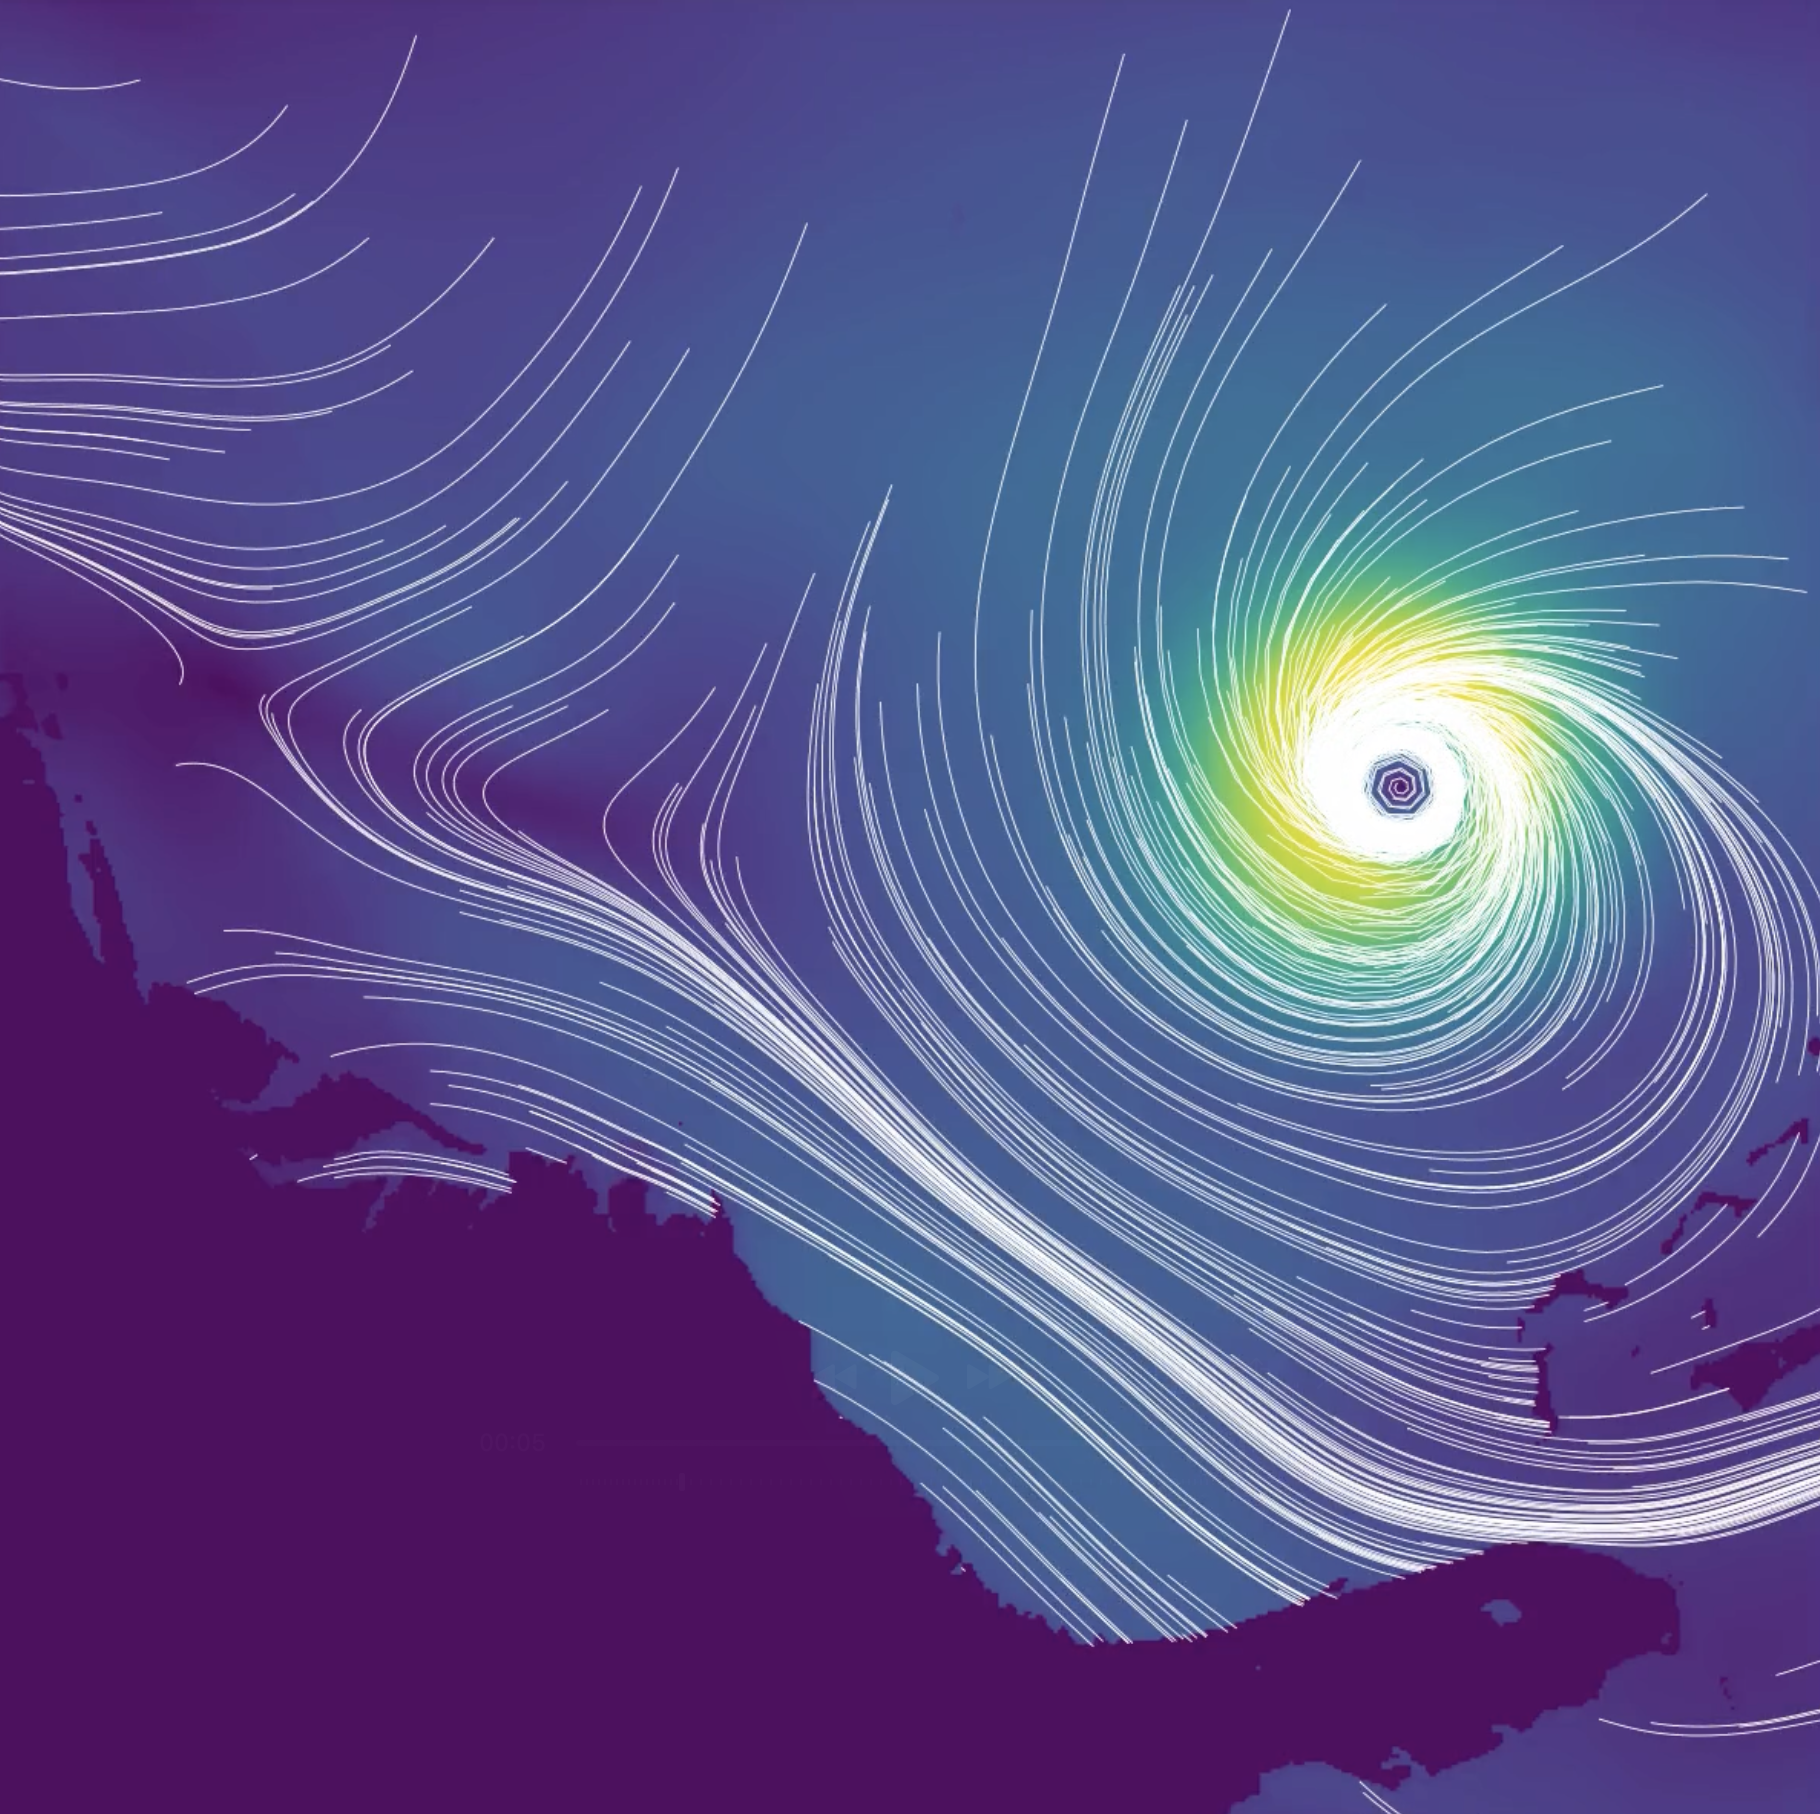
\includegraphics[width=\textwidth, angle=270]{vort_result.png}
        \caption{Field lines from vorticity map with flat bias}
    \end{subfigure}
    \hfill
    \begin{subfigure}{0.43\textwidth}
        \centering
        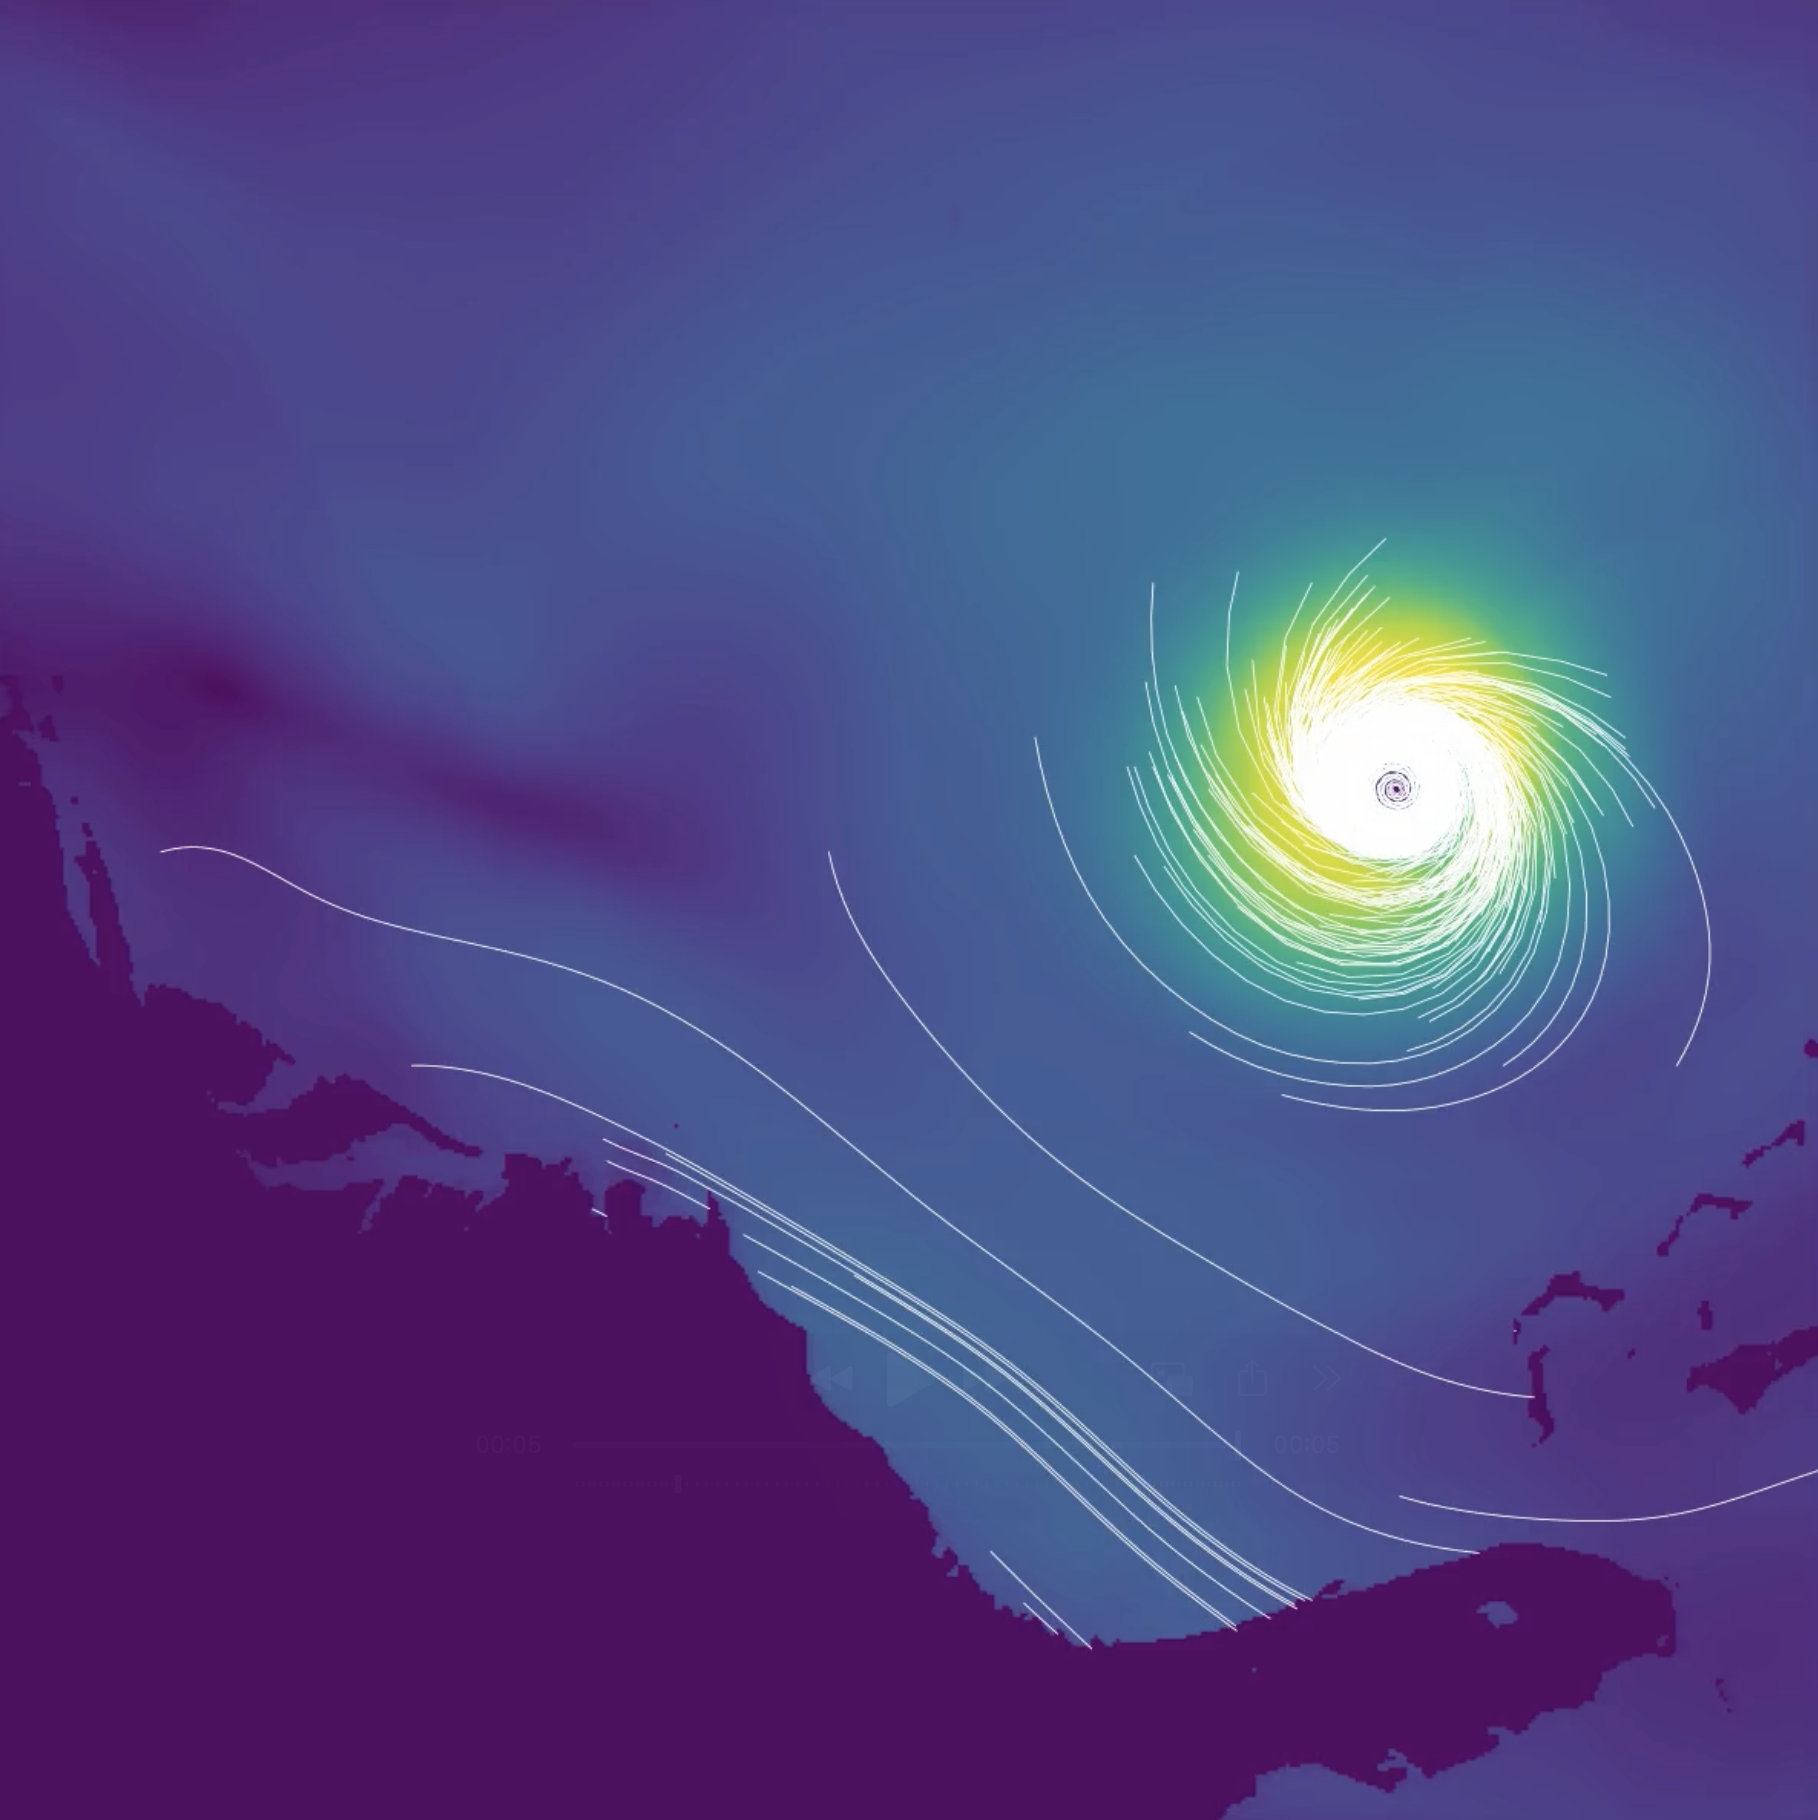
\includegraphics[width=\textwidth, angle=270]{vort_result_3_0.png}
        \caption{Field lines from vorticiy map raised to 3.0}
    \end{subfigure}
    \caption{}
\end{figure}

All three strategies are able to highlight the general structures of the vector field, and it is difficult to say which one
is the most appropriate or useful. Overall, the uniform and random sampling strategies are very easy to implement, but give little control,
and no domain insight is used to highlight particular features. The vorticity-based sampling uses some domain insight (areas with high vorticity are more "interesting"), but
requires more computation and some tweaking to yield good results. Still, this allows for more control in how the sampling is done, and we might
get away with using fewer particles overall, reducing clutter.

The difference in accuracy between euler-forward and RK4 are clear when inspecting the area high in vorticity:
\begin{figure}[h!]
    \centering
    \begin{subfigure}{0.48\textwidth}
        \centering
        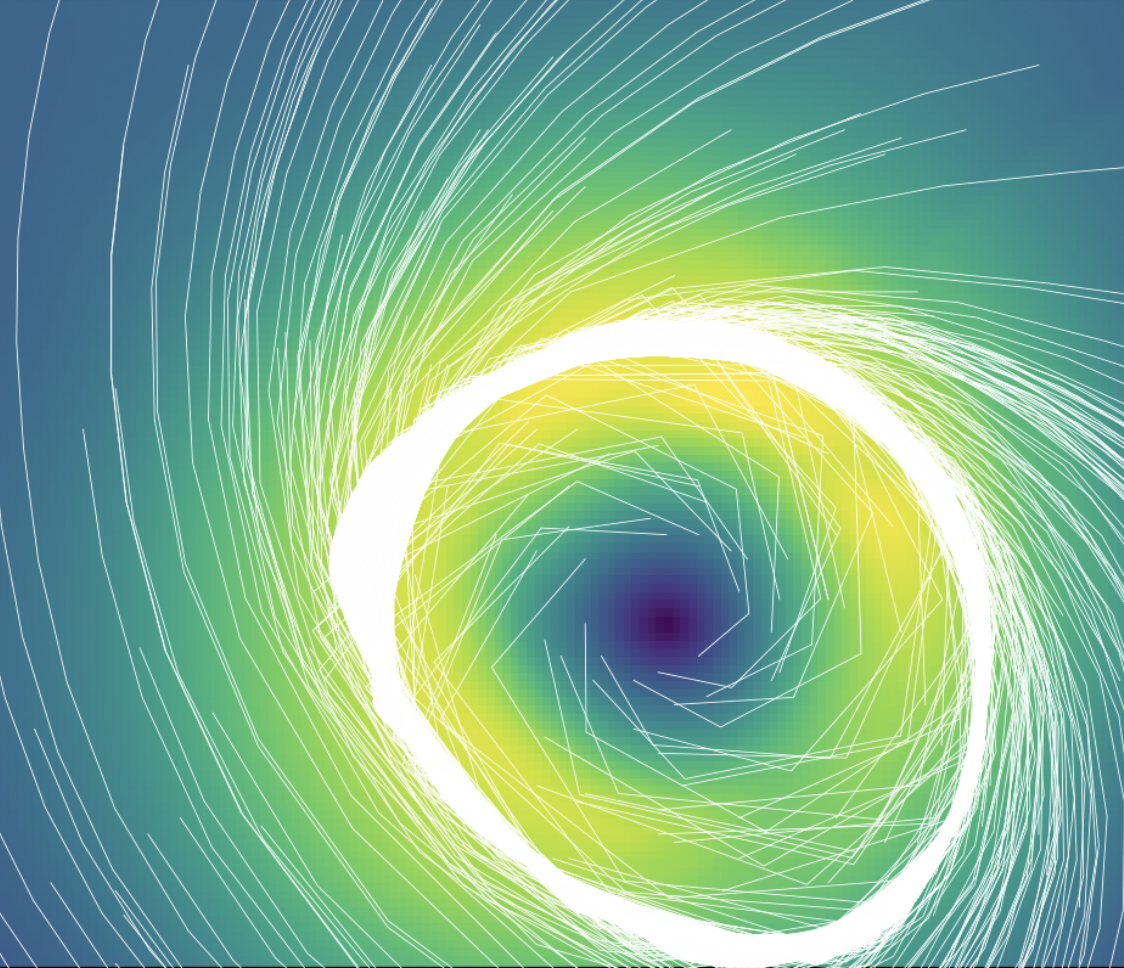
\includegraphics[width=\textwidth, angle=0]{euler.png}
        \caption{Euler}
    \end{subfigure}
    \hfill
    \begin{subfigure}{0.48\textwidth}
        \centering
        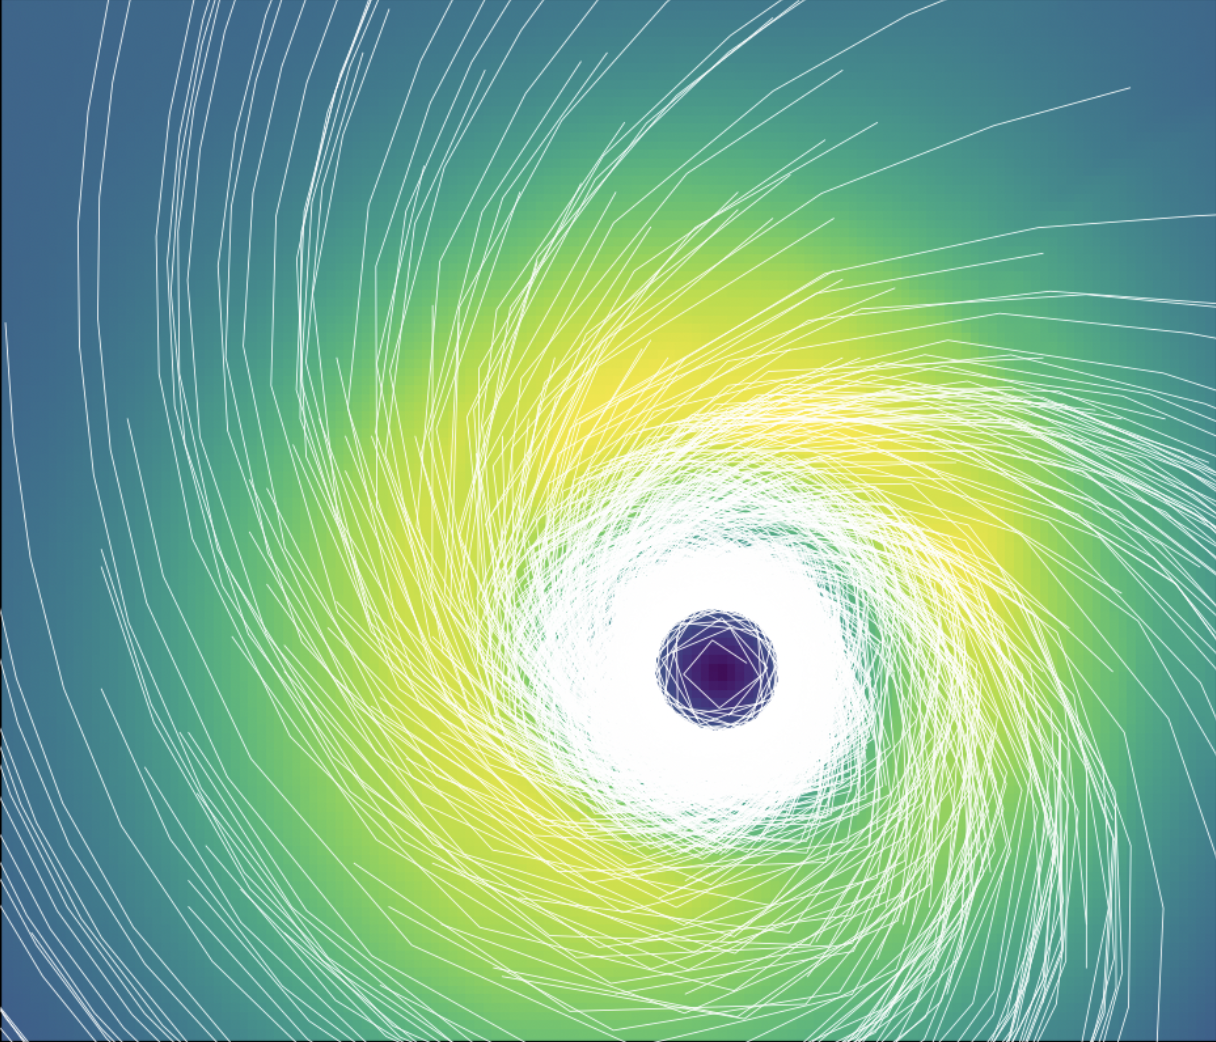
\includegraphics[width=\textwidth, angle=0]{rk4.png}
        \caption{RK4}
    \end{subfigure}
    \caption{}
\end{figure}

\section{Line Integral Convolution}
The LIC algorithm is another method for visualizing vector fields. This method is also based on numerical integration of stream lines,
but does not rely on a seeding strategy. Instead, LIC produces a full visualization at pixel-resolution.

\subsection{Algorithm and implementation}
The same procedure is used to determine the color/intensity of each pixel in the LIC result, which in the simple case is a greyscale image
with resolution equal to the size of the data grid.

The intensity of a pixel $I(u, v)$ is defined as
$$I(u, v) = \int_{-L/2}^{L/2}k(s)N(\sigma_{uv}(s))ds$$
Where L is the kernel length, k is the kernel, N is a noise
texture. $\sigma_{uv}$ is the unique field line passing through the pixel $(u, v)$. Intuitively, each pixel
in the output texture is the result of blurring the noise texture at points along the field line passing through that pixel.
The result is that pixels along the same field line will obtain similar intensities (correlated), while pixels orthogonal to the field line will be uncorrelated.

\newpage

In the implementation, the computation of the field lines themselves and the convolutions with the kernel happen simultaneously.
The computation is separated into a forward-stepping part and a backward-stepping part.
The implementation (forward part only) in pseudo-code:
\begin{verbatim}
x, y = pixel
for {s = 0; s <= L/2; s++}{
    u_local, v_local = velocity(x, y)
    mag_local = sqrt(u_local**2 + v_local**2) 

    dtx = step_size * u_local / mag_local
    dty = step_size * v_local / mag_local
    x += dtx
    y += dty

    output_texture(x, y) += h[s] * noise_texture(x, y)
}

\end{verbatim}
This is a naive and slow implementation of LIC, though relatively simple to implement.
A large inefficiency is that the same field lines are recomputed many times, since many pixels will 
fall coincide with the same stream lines.

\subsection{Results}
As post-processing steps, the LIC image was normalized and histogram equalization was used to increase
the contrast of the LIC image. Then, the LIC image was blended with the velocity magnitude image using the 
LIC image as an intensity map.

First, a fixed kernel size of 8000 was chosen, and LIC images
were produced using different arc lengths:

\begin{figure}[h!]
    \centering
    \begin{subfigure}{0.32\textwidth}
        \centering
        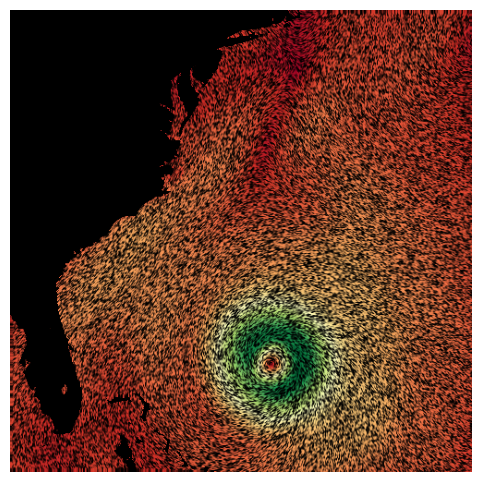
\includegraphics[width=\textwidth]{steps_8000_kernel_length_4.png}
        \caption{arc length = 4}
    \end{subfigure}
    \hfill
    \begin{subfigure}{0.32\textwidth}
        \centering
        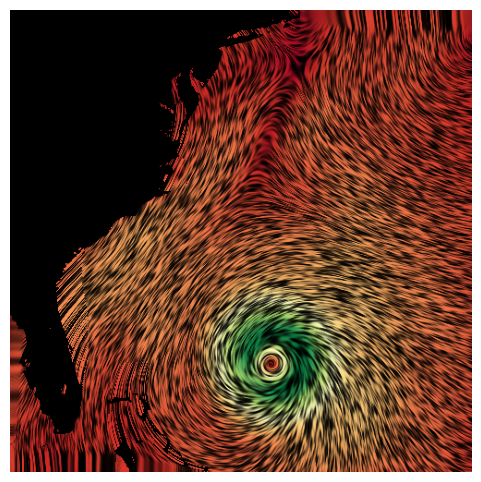
\includegraphics[width=\textwidth]{steps_8000_kernel_length_8.png}
        \caption{arc length = 8}
    \end{subfigure}
    \hfill
    \begin{subfigure}{0.32\textwidth}
        \centering
        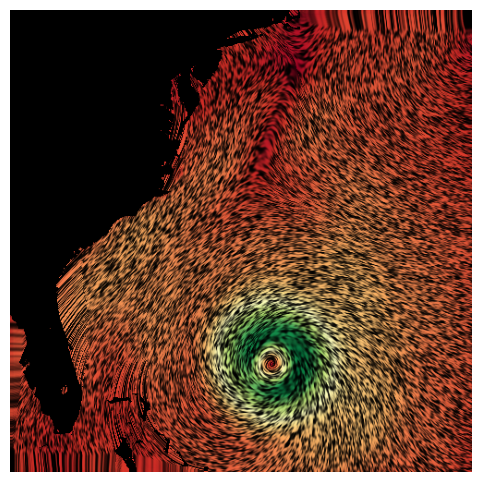
\includegraphics[width=\textwidth]{steps_8000_kernel_length_16.png}
        \caption{arc length = 16}
    \end{subfigure}
    \caption{}
\end{figure}

From these results it is clear that the arc length chosen significantly
changes the quality of the image. For these particular parameters, the result seems to get worse for arc lengths significantly
greater than or less than 8. 

In the second comparison, a constant arc length of 4 was chosen, and different kernel lengths L were tested.

\begin{figure}[h!]
    \centering
    \begin{tabular}{cc}
        \subcaptionbox{L=100}{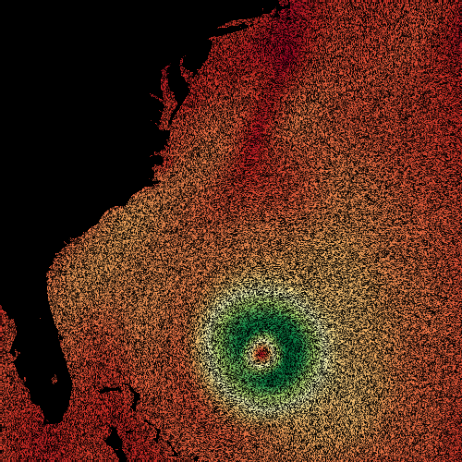
\includegraphics[width=0.45\textwidth]{frame_000.png}} &
        \subcaptionbox{L=2000}{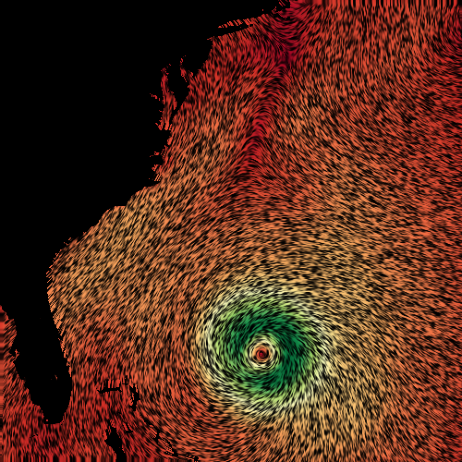
\includegraphics[width=0.45\textwidth]{frame_006.png}} \\
        \subcaptionbox{L=4000}{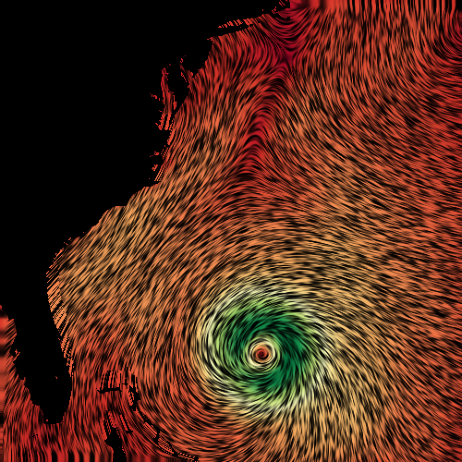
\includegraphics[width=0.45\textwidth]{frame_012.png}} &
        \subcaptionbox{L=6000}{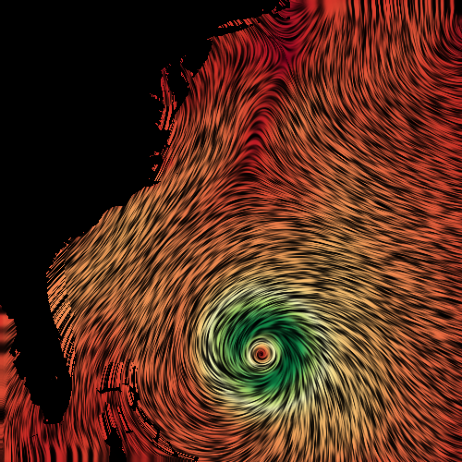
\includegraphics[width=0.45\textwidth]{frame_018.png}} \\
    \end{tabular}
    \caption{LIC with constant arc length and varying kernel size}
\end{figure}

The kernel length determines the accuracy of the field line computations and has a direct impact on the LIC result.
If the kernel length is too low, pixels which are theoretically on the same field lines will find different solutions which reduces
the correlation along the field lines. The larger the kernel size, the stronger correlations will be, though the improvements will diminish as L grows sufficiently large.

\section{Geometric vs. Texture-based Methods}
The accuracy of the numerical integration (Euler vs RK4) is very important in LIC, as even small errors in the solutions found will decrease the coherence in the image.
For LIC to be successful, the pixels which coincide with a given analytical field line must compute arcs that mostly lie on this line. While accuracy is important
for line-based methods as well, one can get acceptable line-based visualizations even with relatively inaccurate solvers.

Line-based methods are also more intuitive than LIC, though care must be taken in choosing the right seeding strategy. With line-based methods, it's easy to miss
important structures in the data, as large areas of the vector field are totally disregarded. LIC is more complete in this sense, where strong features and critical points
appear naturally through evaluating the entire field/all pixels.

In general, both methods can produce satisfying visualizations of vector fields, and they are
both very flexible. In line-based visualization, a plethora of seeding strategies can be used to produce different results.
In LIC, different input textures, kernel sizes and sub-arc lengths can be experimented with.

Both methods are easily parallellizable as the same algorithm is used for all elements (seeds for lines, pixels for LIC). In terms of performance, the geometric method
was faster in these experiments, but it should be noted that the LIC algorithm implemented is very slow and can be optimized.

\section{Summary and Conclusion}
This report explored methods for visualizing vector fields using field lines and Line Integral Convolution (LIC). Various seeding strategies were tested for field lines: random, uniform, and vorticity-based seeding. Numerical integration methods, Euler and RK4, were compared, with RK4 being more accurate especially regions of high vorticity.

LIC was implemented as a texture-based approach, producing a dense, high-resolution visualization. The effects of kernel length and arc length were examined, demonstrating their influence on image quality. Compared to field lines, LIC provides a more complete visualization but requires higher computational effort.


\section*{Links to code}
Line integral convolution: https://github.com/edvartGB/visualization/blob/main/oblig/lic_vectorized.ipynb

Stream lines: 


\end{document}
